\documentclass[11pt]{article}
\usepackage[sc]{mathpazo} %Like Palatino with extensive math support
\usepackage{fullpage}
\usepackage[authoryear,sectionbib,sort]{natbib}
\linespread{1.7}
\usepackage[utf8]{inputenc}
\usepackage{lineno}
\usepackage{titlesec}
% Added later
\usepackage{amsmath}  % for equations
\usepackage{graphicx} % for figures
\titleformat{\section}[block]{\Large\bfseries\filcenter}{\thesection}{1em}{}
\titleformat{\subsection}[block]{\Large\itshape\filcenter}{\thesubsection}{1em}{}
\titleformat{\subsubsection}[block]{\large\itshape}{\thesubsubsection}{1em}{}
\titleformat{\paragraph}[runin]{\itshape}{\theparagraph}{1em}{}[. ]\renewcommand{\refname}{Literature Cited}

\usepackage{color}
	\definecolor{darkred}{rgb}{0.75,0.1,0.1}
	 \definecolor{darkblue}{rgb}{0,0,0.75}
	 \definecolor{magenta}{rgb}{0,0,0.75}
\newcommand{\cha}[1]{\textcolor{darkred}{(#1)}}

\usepackage{hyperref}
\definecolor{darkgreen}{rgb}{0.1,0.6,0.3}
\hypersetup{
    colorlinks=true,       % false: boxed links; true: colored links
    linkcolor=blue,          % color of internal links (change box color with linkbordercolor)
    citecolor=darkgreen,        % color of links to bibliography
    filecolor=magenta,      % color of file links
    urlcolor= black           % color of external links
}
%%%%%%%%%%%%%%%%%%%%%
% Line numbering
%%%%%%%%%%%%%%%%%%%%%
%
% Please use line numbering with your initial submission and
% subsequent revisions. After acceptance, please turn line numbering
% off by adding percent signs to the lines %\usepackage{lineno} and
% to %\linenumbers{} and %\modulolinenumbers[3] below.
%
% To avoid line numbering being thrown off around math environments,
% the math environments have to be wrapped using
% \begin{linenomath*} and \end{linenomath*}
%
% (Thanks to Vlastimil Krivan for pointing this out to us!)

\title{Multiple infections and complex life cycles}

% This version of the LaTeX template was last updated on
% November 8, 2019.

%%%%%%%%%%%%%%%%%%%%%
% Authorship
%%%%%%%%%%%%%%%%%%%%%
% Please remove authorship information while your paper is under review,
% unless you wish to waive your anonymity under double-blind review. You
% will need to add this information back in to your final files after
% acceptance.

\author{Phuong Linh Nguyen$^{1,\ast}$ \& 
Chaitanya S. Gokhale$^{2}$
}
\date{}

\begin{document}
%\linenumbers
\maketitle

%
\noindent{} $^1$Theoretical Ecology and Evolution Group, Department of Biology, University of Fribourg, Switzerland
\noindent{} $^2$Research Group for Theoretical Models of Eco-evolutionary Dynamics, Department of Evolutionary Theory, Max Planck Institute for Evolutionary Biology, Pl\"{o}n 24306, Germany;
%
\noindent{} $\ast$ Corresponding author; e-mail: linh.phuong.nguyen@evobio.eu

\bigskip

\textit{Manuscript elements}:  Figure~1, figure~2, figure~3, figure~4, figure~5, figure~6, % appendices~A and B (including figure~A1, figure~B1 and figure~B2). All figures except figure~3 are in color.

\bigskip

\textit{Keywords}: host manipulation, multiple infections


\bigskip

\textit{Manuscript type}: e-article. %Or e-article, note, e-note, natural history miscellany, e-natural history miscellany, comment, reply, invited symposium, or historical perspective.

\bigskip

\noindent{\footnotesize Prepared using the suggested \LaTeX{} template for \textit{Am.\ Nat.}}

\linenumbers{}
%\modulolinenumbers[3]

\newpage{}

\section*{Abstract}
Host manipulation is a common strategy of parasites of different complexity. 
Host manipulation directly affects predator-prey dynamics in trophically transmitted parasites, where parasite transmission requires predation. Theoretical studies suggest that manipulation that enhances predation often results in a heavy burden on the prey population. 
Consequently, the system is often destabilised, leading to parasites prone to extinction. 
Host manipulation, however, can also suppress predation.
Such suppression is possible if multiple parasites coinfect a host with conflicting interests in manipulation. 
The interests could be misaligned for various reasons, such as limited carrying capacity or parasitoid developmental stage.
Multiple infections are a norm in parasite ecology but are often neglected in the theoretical assessment of host-parasite dynamics.
We tease apart the effect of host manipulation of coinfected parasites and manipulation interests via a mathematical model of a trophically transmitted parasite with a complex life cycle.
The life cycle comprises a free-living state, an intermediate and a definitive host. 
With coinfection, we show that host manipulation that enhances predation need not always destabilise the predator-prey system. 
However, cooperation between coinfected parasites leading to increased predation and can lead to bistability such that a slight disturbance in the system drives the parasite population to extinction. 
On the other hand, when coinfected parasites sabotage the manipulative ability of one another, the stability of the predator-prey system is always guaranteed.
Our study highlights the necessity and means of incorporating the reality of multiple parasites and their multi-trophic life cycles in a single system in studying parasite ecology.

\newpage{}

\section*{Introduction}

% The journal does not have numbered sections in the main portion of
% articles. Please refrain from using section references (à la
% section~\ref{section:CountingOwlEggs}), and refer to sections by name
% (e.g. section ``Counting Owl Eggs'').

Parasites infect life on earth ubiquitously, and many of these parasites have complex life cycles \citep{zimmer:book:2001}. 
While a complex lifecycle can be defined as abrupt ontogenic changes in morphology and ecology \citep{Benesh:2016dj}, a complex parasitic lifecycle typically involves numerous hosts that a parasite needs to traverse to complete its life cycle. 
This complex lifecycle results in the evolution of various strategies that enable the success of parasite transmission from one host to another. 
One famous strategy that inspires many science fiction movies and novels is host manipulation, where a parasite can alter the morphology and/or behaviour of its  host to enhance its transmission to the next host \citep{Hughes2012}. 
Host manipulation has been shown in many host-parasite systems, from parasites with simple life-cycle to those with complex life-cycle that involves more than one host \citep{Hughes2012,molyneux1986}. 
For instance, sand flies infected by \textit{Leishmania} parasites bite more and take more time for a blood meal from mammals (the definitive host of \textit{Leishmania}) compared to their uninfected counterparts \citep{Rogers2007}. 
Copepods infected by cestode parasites are more active and accessible to sticklebacks (the definitive hosts of the cestodes) compared to uninfected copepods \citep{Wedekind1996}.

Theoretical studies have long attempted to understand the ecological and evolutionary consequences of host manipulation. 
\cite{Roosien2013} and \cite{Hosack2008} showed that manipulative parasites could increase the disease prevalence in an epidemic. Evolutionarily, \cite{Gandon2018} studied the evolution of the manipulative ability of infectious disease parasites, showing different evolutionary outcomes depending on whether the pathogen can control its vector or host.
\cite{Hadeler1989, Fenton2006} and \cite{Rogawa2018} showed that host manipulation could stabilise or destabilise the predator-prey dynamics depending on how manipulation affects the predation response function and the assumption on the fertility of the definitive infected host. \cite{Seppl2008} showed that host manipulation could evolve even when it increases the risk of the intermediate host being eaten by a non-host predator, given that the initial predation risk is sufficiently low. 
These models, however, lack a crucial aspect of parasite dynamics, multiple infections. 
Typical studies do not consider multiple infections, a phenomenon that is the norm rather than an exception in parasitism. 
Multiple infections result in the coinfection of more than one parasite inside a host, which may alter the manipulative outcomes. 
An alignment of interest between coinfecting parasites may enhance manipulation, while a conflict of interest may reduce the manipulative effect. 
Indeed, \cite{Hafer:2015gl} showed that copepods infected by two cestode parasites reduce the activity of copepods when both parasites are at the same noninfectious stage, i.e. both parasites are not ready to transmit. 
Thus the reduction in mobility is suggested to reduce the predation rate by the definitive hosts. 
When two infectious parasites infect the copepods, the copepods' activity increases, and so does the predation risk for the copepod. 
However, when the copepods are infected by one infectious and one noninfectious parasite, their interests clash, and one parasite wins over the other. 

\begin{figure}[ht!]
\centering
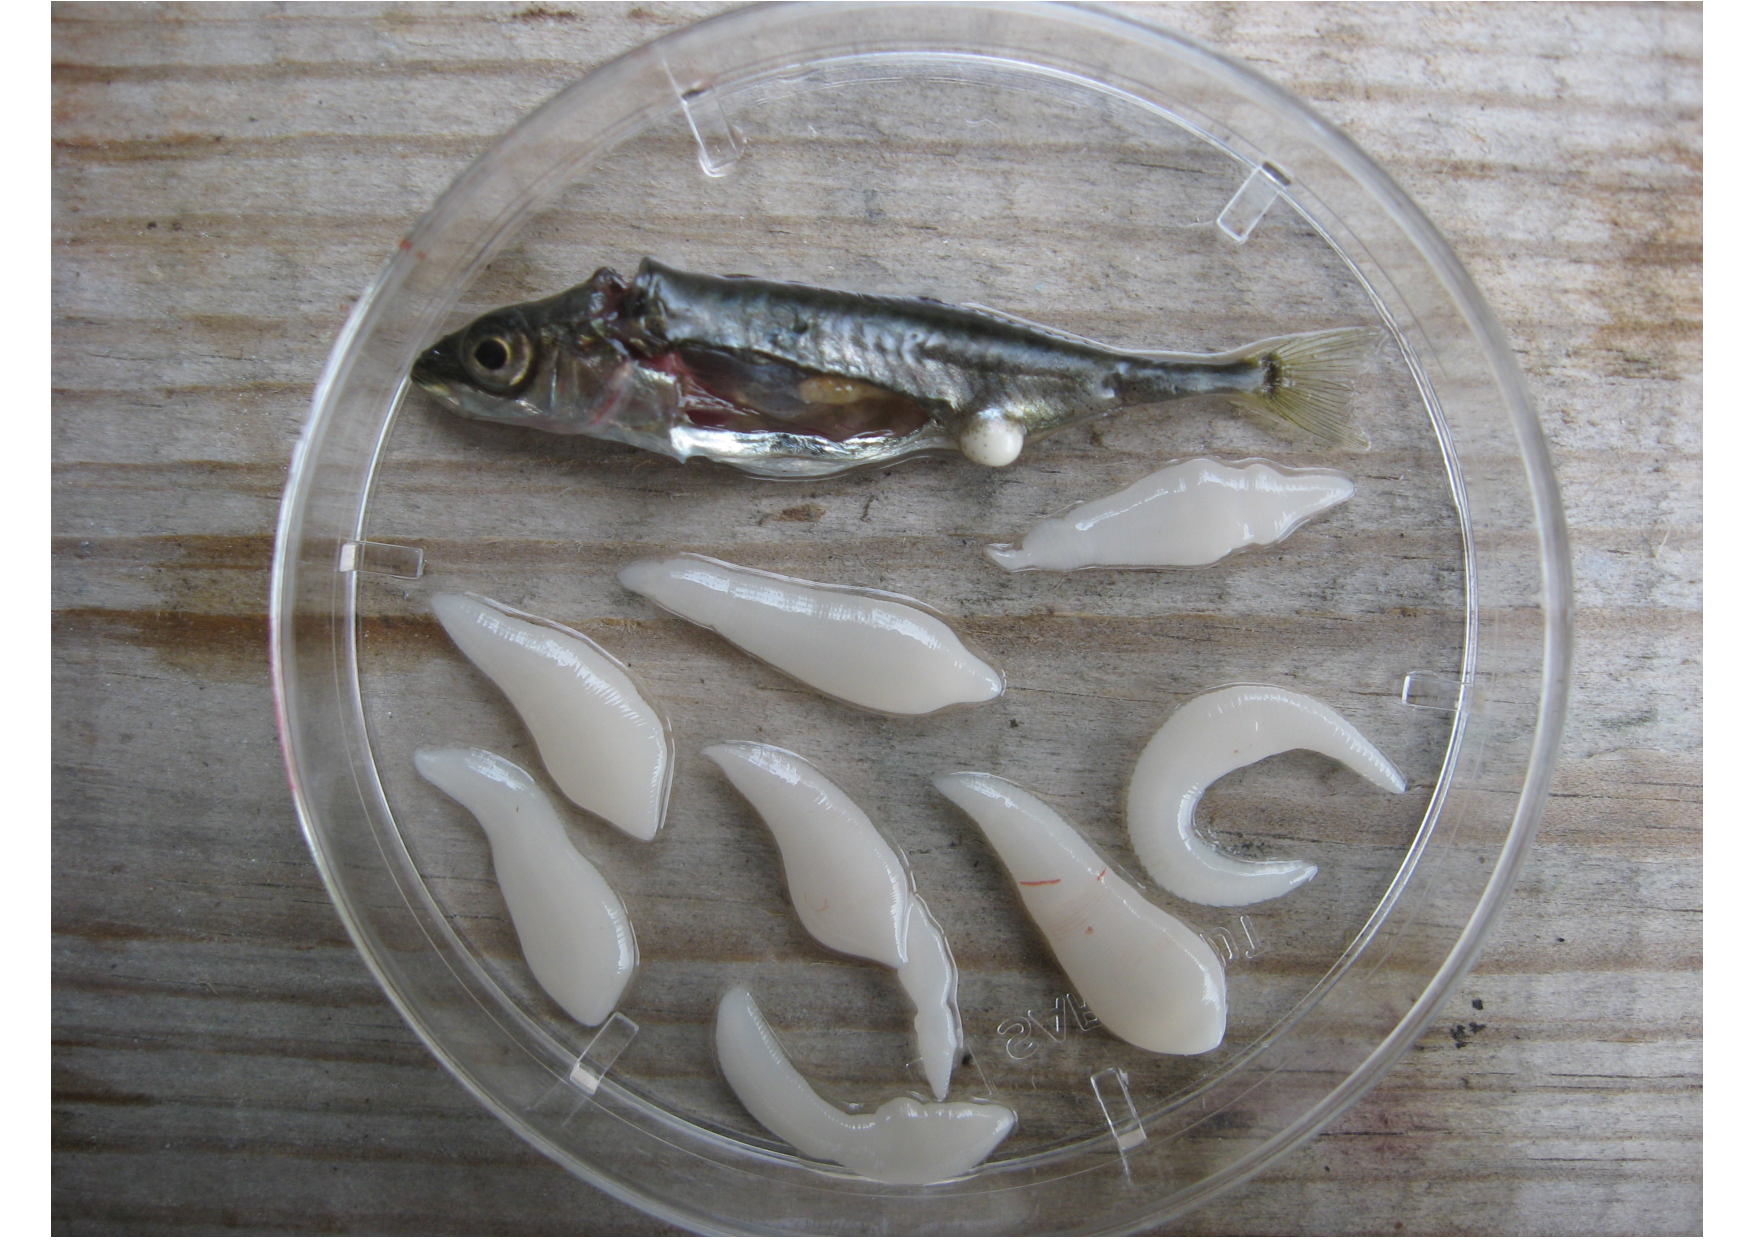
\includegraphics[width=0.75\columnwidth]{Figures/Sept_10_ 101.pdf}
\caption{\textbf{Who is in control?.}
Schistocephalous eggs, which overwinter at the bottom of bodies of water, hatch into microscopically small swimming larvae. 
These larvae are eaten by copepods (also known as Cyclops due to its single eye), where they develop to the second larval stage. 
However, the copepod is only the first intermediate host. 
The larvae are then eaten by sticklebacks, where they reach the third larval stage and grow significantly in size and weight. 
For the parasite to successfully reach its final host, a warm-blooded animal like a bird, it manipulates its intermediate hosts. 
The timing is crucial as the chances of success are greatest if the larvae develop in the copepod for 13 to 15 days before entering the stickleback. 
The presence of multiple parasites in the same host can lead to competition and strategic decision pertaining to investment in manipulation and growth.
And indeed a stickleback can be infected by numerous tapeworms as shown above by Martin Kalbe.
}
\label{fig:schematic}
\end{figure}


Theoretical work that considers multiple infections often focuses on the evolution of virulence \citep{vanBaalen1995, Alizon2013, Alizon2008, Choisy2010, Alizon2012}. 
They show that multiple infections can lead to an increase in virulence \citep{vanBaalen1995, Choisy2010}, a branching of one less virulent and one hypervirulent parasite when within-host dynamics are considered \citep{ Alizon2008}, a reduction in virulence if parasites are co-transmitted \citep{Alizon2012}. 
In epidemiological models, higher virulence is often assumed to link with a higher transmission rate; virulence is therefore associated with host manipulation in such cases. 
In trophically transmitted parasites, host manipulation influences the predation rate, which predominantly affects predator-prey dynamics. 
Theoretical studies on host manipulation in trophically transmitted parasites with multiple infections are rare \citep{Parker2003,Vickery2009}. Moreover, they do not consider the prey-predator dynamics, which is likely to have important feedback on the evolution of host manipulation. 
A few studies that consider the prey-predator dynamics do not incorporate multiple infections \citep{Rogawa2018, Iritani2018, Hadeler1989, Fenton2006}. 
More importantly, they assume that transmission from definitive hosts to intermediate hosts is due to direct contact between the two types of hosts. 
This is often not the case, as parasites are released from the definitive hosts into the environment. 
Transmission happens only when intermediate hosts have contact with this free-living parasite pool.


Our study addresses the gap in the theoretical work on host manipulation in trophically transmitted parasites.
We include multiple infections and consider the dynamics of the free-living parasite pool. 
We use a compartmental model that illustrates a complex lifecycle parasite with two hosts: an intermediate host preyed upon by a definitive host. 
Transmission from the intermediate host to the definitive host occurs when predation on infected intermediate hosts happens. 
Reproduction only happens in the definitive hosts. 
New parasites are then released into the environment, where they again have contact with the intermediate hosts to complete their lifecycle. 
We focus on the manipulation of the intermediate hosts, such that the parasite increases the predation rate on the intermediate host by the definitive host to increase its transmission rate. 
We then analyse the effect of host manipulation on the ecological dynamics of the prey-predator-parasite system. 
We found that cooperation in host manipulation leads to bistability in the predator-pray system, given that reproduction from multiple infections is sufficiently high. 
This suggests that disturbance in the system may result in parasite extinction. 
Sabotage in host manipulation, however, always guarantees unique stable equilibrium in the system. 

\section*{Model and Results}

Our model concerns the complex lifecycle of a trophically transmitted parasite that requires two hosts: an intermediate host and a definitive host. 
Reproduction only happens inside the definitive hosts and new parasitic progeny are released in to the environment. 
An intermediate host can be infected if it encounters this free-living parasite pool. 
Finally, when a definitive host consumes an infected intermediate host, the definitive host gets infected, and the parasite completes its lifecycle.


For simplicity, we assume that hosts can be infected by one (single infection) or, at most, two parasites (double infections). 
Our model is therefore more close to macro-parasitic system.
Given that infection occurs, the probability that two parasites from the parasite pool co-transmit to an intermediate host is denoted by  $p$, and thus $1-p$ is the probability that a single parasite enters an intermediate host. 
When a definitive host consumes an intermediate host infected by two parasites, there is a probability $q$ that the parasites co-transmit to the definitive host.
With probability $1-q$, only one parasite successfully transmits. 
This formulation assumes that infection always happens when hosts encounter parasites.
The dynamics of a complex lifecycle parasite that requires two hosts is described by the following system of ODEs, firstly for the intermediate host as,
%
\begin{align}
\frac{dI_s}{dt} &= R(I_s, I_w, I_{ww}) - d I_s - P_s(D_s, D_w, D_{ww}) I_s  - \eta  I_s \nonumber \\ 
\frac{dI_w}{dt} &=  (1 - p) \eta I_s  - (d + \alpha_w) I_w - P_w(D_s, D_w, D_{ww}, \beta_w) I_w \label{odes:ihosts} \\
\frac{dI_{ww}}{dt} &= p \eta I_s  - (d + \alpha_{ww}) I_{ww} - P_{ww}(D_s, D_w, D_{ww}, \beta_{ww}) I_{ww} \nonumber
\end{align}
%
where $R(I_s, I_w, I_{ww})$ represents the birth rate of the intermediate hosts, a function of both infected and uninfected individuals.
$P_s, \ P_w, \ P_{ww}$ are the predation functions of definitive hosts on  respectively susceptible, singly infected and doubly infected intermediate hosts. 
The predation function depends on the density of the definitive hosts and the manipulative strategies of parasites in the intermediate hosts. 
In particular, if a single parasite infects an intermediate host, the manipulation strategy is $\beta_w$. 
However if the intermediate host is co-infected, the manipulation strategy is $\beta_{ww}$. 
In the scope of this model, we assume no link between $\beta_w$ and $\beta_{ww}$ to explore all possible ecological outcomes of the system. 
The force of infection by parasites in the environment is denoted by $\eta = \gamma W$. 
The force of infection that corresponds respectively to singly infected intermediate host ($I_w$), and doubly infected intermediate hosts ($I_{ww}$) is denoted respectively by $\lambda_w = \beta_w I_w$ and $\lambda_{ww} = \beta_{ww} I_{ww}$. 
Because in reality parasites can manipulate both intermediate and definitive hosts, here, whenever we mention host manipulation, it specifically refers to the manipulation in intermediate hosts, which correlates to the predation rate.

For the definitive hosts we have,
\begin{align}
\frac{dD_s}{dt} &= B(D_s,  D_w,  D_{ww},  I_s, I_w, I_{ww})  - \mu D_s - (\lambda_{ww} + \lambda_w) D_s \nonumber \\    
\frac{dD_w}{dt} &= (\lambda_w + 2 (1 - q) \lambda_{ww}) D_s - (\mu + \sigma_w) Dw - (2 (1 - q) \lambda_{ww} + \lambda_w) D_w  \label{odes:dhosts} \\         
\frac{dD_{ww}}{dt} &= q \lambda_{ww} D_s + (2 (1 - q) \lambda_{ww} + \lambda_w) D_w - (\mu + \sigma_{ww}) D_{ww} \nonumber
\end{align}
%
where $B(D_s, D_w, D_{ww}, I_s, I_w, I_{ww})$ represents the birth rate of definitive hosts, which depends on the density of both intermediate and definitive hosts, infected or uninfected alike. 
The dynamics of the free-living parasites in the environment are then given solely by,
\begin{align}
	\frac{dW}{dt} &= f_w D_w + f_{ww} D_{ww} - \delta W - \eta I_s \label{odes:eparasite}
\end{align}
%
Definitions of different parameters can be found in Table~\ref{table:varpardescription}.
%
\begin{table}[!ht]
\begin{tabular}{|p{2.5cm}|p{12cm}|} 
\hline
Parameters and Variables    &  Description  \\
\hline
$I_i$  & Density of intermediate hosts that are susceptible $i=s$, singly infected $i=w$, or doubly infected $i=ww$ \\
\hline
$D_i$ & Density of definitive hosts that are susceptible $i=s$, singly infected $i=w$, or doubly infected $i=ww$ \\
\hline
$W$ & Density of parasites released from definitive hosts into the environment \\
\hline
$d$ & Natural death rate of intermediate hosts \\
\hline
$\alpha_i$ & Additional death rate of intermediate hosts due to infection by a single parasite ($i = w$) or two parasites ($i = ww$) \\
\hline
$p$ & Probability that two parasites cotransmit from the environment to an intermediate host \\
\hline
$\gamma$ & Transmission rate of parasites in the environment to intermediate hosts \\
\hline
$\mu$ & Natural death rate of definitive hosts \\
\hline
$\sigma_i$ & Additional death rate of definitive hosts due to infection by a single parasite ($i = w$) or two parasites ($i = ww$) \\
\hline
$\sigma_i$ & Additional death rate of the hosts due to being infected by a singly parasite ($i = w$) or two parasites ($i = ww$) \\
\hline
$q$ & Probability that two parasites cotransmit from intermediate hosts to definitive hosts \\
\hline
$\beta_i$ & Transmission rate of parasites from intermediate hosts to definitive hosts \\
\hline
$f_i$ & Reproduction rate of parasites in singly infected definitive hosts ($i = w$) or doubly infected hosts ($i = ww$)\\
\hline
$\delta$ & Natural death rate of parasites in the environment \\
\hline
\end{tabular}
\caption{Description of variables and parameters}
\label{table:varpardescription}
\end{table}

Here, we focus on the manipulation that enhance transmission from intermediate hosts to definitive hosts, we thus simplify the transmission from the parasite pool to intermediate hosts, such that no sequential infection occurs at this transmission state. 
Sequential infection can happen when parasites transmit from intermediate hosts to definitive hosts. 
Therefore, a singly infected definitive host can be further infected by another parasite if it consumes infected intermediate hosts. 
The dynamics of the system are illustrated in figure (\ref{fig:schematic}).

\begin{figure}[ht!]
\centering
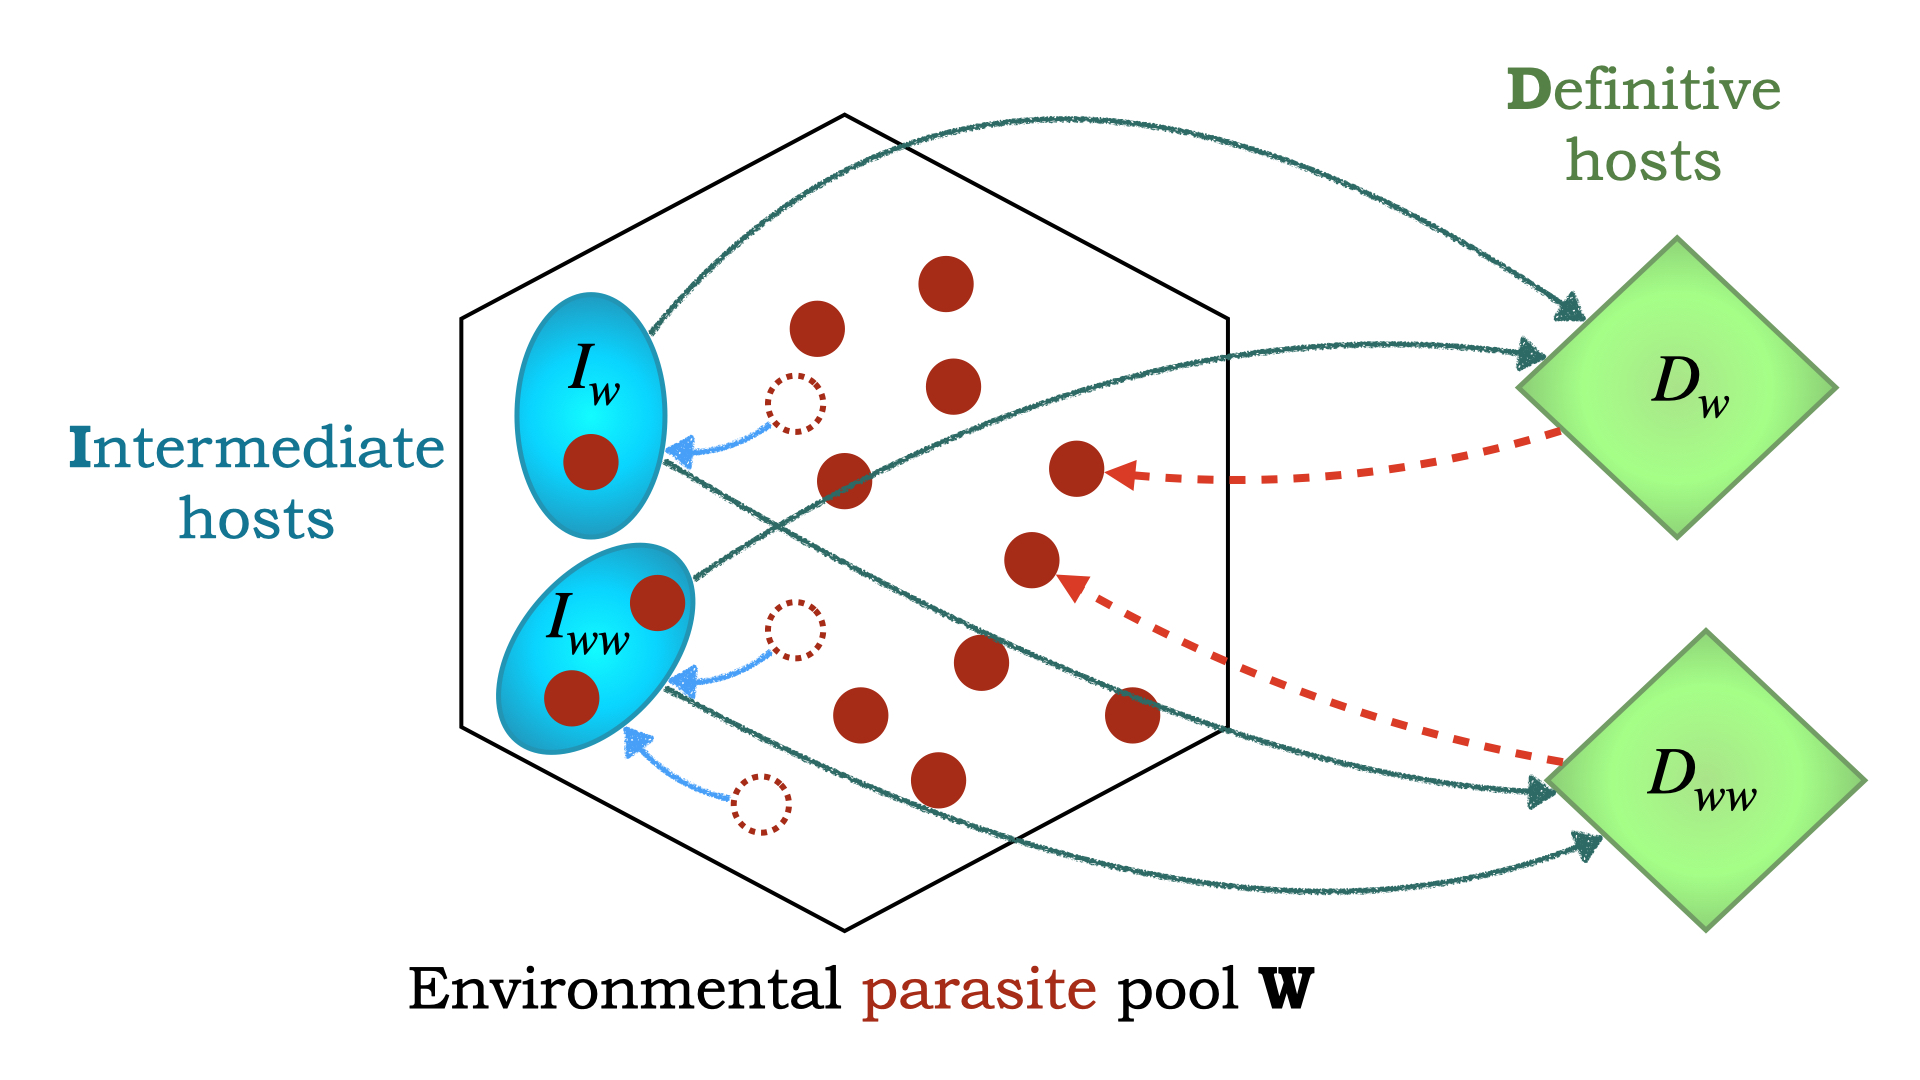
\includegraphics[width=\textwidth]{Figures/schematic.jpeg}
\caption{Schematic of the model. Blue ovales represent intermediate host compartment, 
green diamonds represent definitive host compartment, 
and the transparent hexagon represents the parasite pool compartment with red circles illustrating individual parasites.
}
\label{fig:schematic}
\end{figure}

\subsection*{Basic reproduction ratio $R_0$}

The basic reproduction ratio $R_0$ (or basic reproduction number as often used in epidemiology) is an indication of parasite fitness. 
It can be understood as the expected number of offspring a parasite produces during its lifetime when introduced to a susceptible host population. 
We calculate the basic reproduction ratio $R_0$ using the next-generation method \citep{Diekmann1990, Diekmann2009, Hurford2009} (See SI for details).

\begin{align}
R_0 = & \gamma I_s^* \frac{ p q \beta_{ww}}{\alpha_{ww} + d + P_{ww}} \frac{D_s^*}{\mu +\sigma_{ww}} \frac{f_{ww}}{\delta +\gamma I_s^*} + \nonumber \\
& \gamma  I_s^* \left( \frac{ (1-p)\beta_w}{\alpha_w + d + P_w} + \frac{2 p (1-q) \beta_{ww}}{\alpha_{ww} + d + P_{ww}} \right) \frac{D_s^*}{\mu + \sigma_w} \frac{f_w}{\delta +\gamma  I_s^*}
\end{align}

where $I_s^*$ and $D_s^*$ are the densities of susceptible intermediate and definitive hosts at the disease-free equilibrium. 
Here, the expression of $R_0$ contains possible reproduction routes of a parasite, which can be via double or single infections. 
The first component corresponds to the double infections route, in which the focal parasite co-transmit with another parasite into a susceptible intermediate host, then co-transmits into a susceptible definitive host and reproduces. 
Note that when introduced in a disease-free environment, parasites are so rare that only cotranmission matters where as the compartments with sequential infections are negligible. 
The second component corresponds to the single infection route, wherein the focal parasite infects a susceptible intermediate host via single or double infections. 
The parasite then transmits alone into the susceptible definitive host and eventually reproduces. 


If $R_0 > 1$, a parasite spreads when introduced into the disease-free equilibrium of prey and predator.
Intuitively, the higher the density of susceptible intermediate and definitive hosts, the larger the value of $R_0$ as the infection reservoir is more extensive. 
In contrast, regardless of the explicit form of the predation function, the higher the predation rate $P_w$ and $P_{ww}$, the lower the value of $R_0$ given the smaller reservoir of intermediate hosts. 
The effect of host manipulation on the value of $R_0$ is not so straightforward; as host manipulation becomes more efficient, the transmission rate from the intermediate host to the definitive host increases, but so does the predation rate. 
A higher predation rate results in a smaller intermediate host reservoir for parasites to infect. 
To understand the effect of manipulation on the fitness of parasites and the ecological dynamics of the system, we need to specify the predation functions. 
For simplicity, we consider linear functions for predation,
%
\begin{align*}
& P_s(D_s + D_w + D_{ww}) = \rho D_{total}  \\
& P_w(D_s, D_w, D_{ww}, \beta_w) = (\rho + \beta_w) D_{total} \\
& P_{ww}(D_s, D_w, D_{ww}, \beta_{ww}) =  (\rho + \beta_{ww})D_{total}
\end{align*}
%
where $D_{total} = D_s + D_w + D_{ww}$ is the total density of the definitive hosts, and $\rho$ is the baseline capture rate of the predator on the prey. If an intermediate hosts is infected, it is captured by the definitive hosts with rate $\rho + \beta_w$ if it is singly infected, and with rate $\rho + \beta_{ww}$ if it is doubly infected. Zero values for $\beta_w$ and $\beta_{ww}$ suggest no manipulation. 

For simplicity, we also consider a linear function of the birth of definitive hosts
%
\begin{align*}
B(D_s, D_w, D_{ww}, I_s, I_w, I_{ww}) = \rho c D_{total} I_{total}
\end{align*}
%
where $c$ is the efficiency of converting prey into predator's offspring, and $I_{total} = I_s + I_w + I_{ww}$ is the total density of the intermediate hosts.
The birth rate of the predators depends on the capture rate, but it is not affected by host manipulation as,to our best knowledge, there is no supporting evidence.

The explicit form of $I_s^*$ and $D_s^*$ depends on the precise form of all birth and predation functions $B, R, P_s, P_w$ and $P_{ww}$.
But, it does not depend on the manipulation ability or any other parameter of the parasite. 
$I_s^*$ and $D_s^*$ represent the prey-predator dynamics when there is no parasite. 
Given that the birth rate of the predator and the predation rate are linear functions concerning the prey and predator density, the form of the birth rate $R$ of the prey, therefore, has a significant effect on the susceptible intermediate and definitive host dynamics.

\subsection*{Linear birth function of intermediate hosts}
Here, we consider the system when the birth function $R$ of the intermediate host is linear, specifically, $R(I_s, I_w, I_{ww}) = r I_{total}$. 
The equilibrium of intermediate and definitive hosts in the disease-free state are,
%
\begin{align*}
& I_{s0}^* = \frac{\mu}{c \rho} \\
& D_{s0}^* = \frac{r - d}{\rho}
\end{align*}
%
This equilibrium is always unstable. 
In particular, it has a cyclic behaviour because, at this equilibrium, the jacobian matrix of the system (\ref{odes:ihosts}, \ref{odes:dhosts}, \ref{odes:eparasite}) always has one imaginary eigenvalue with a positive real part. 
This follows from the Lotka-Volterra system using linear functions for prey birth and predation \citep{Lotka1920}.
Because the disease-free dynamics is cyclic, it is difficult to analyse the spread of a parasite (often evaluated when the disease-free state is stable). 
Here,  $R_0 > 1$  happens when $\gamma$, the transmission rate from the environment to intermediate hosts, and $f_w, f_{ww}$, the reproduction of the parasites are greater than a threshold (see supplementary ). 
However, even when this condition is satisfied, the parasite may not be able to spread and persist in cyclic susceptible host dynamics (Figure \ref{fig:diseasefree:linear}). 
This result agrees with the conclusion in \citep{Ripa:Evol:2013}, which suggests that it is difficult for a mutant to invade a cyclic population. 
In our case, it is not the invasion of a mutant but the spread of a parasite in a cyclic disease-free host population, but the argument remains valid in both cases. 
This issue deserves a more thorough investigation, which is out of the scope of this article. 
We, therefore, choose a non-linear birth function of the intermediate hosts to obtain a stable disease circulation state and focus on the effect of host manipulation on the ecological dynamics. 

\begin{figure}
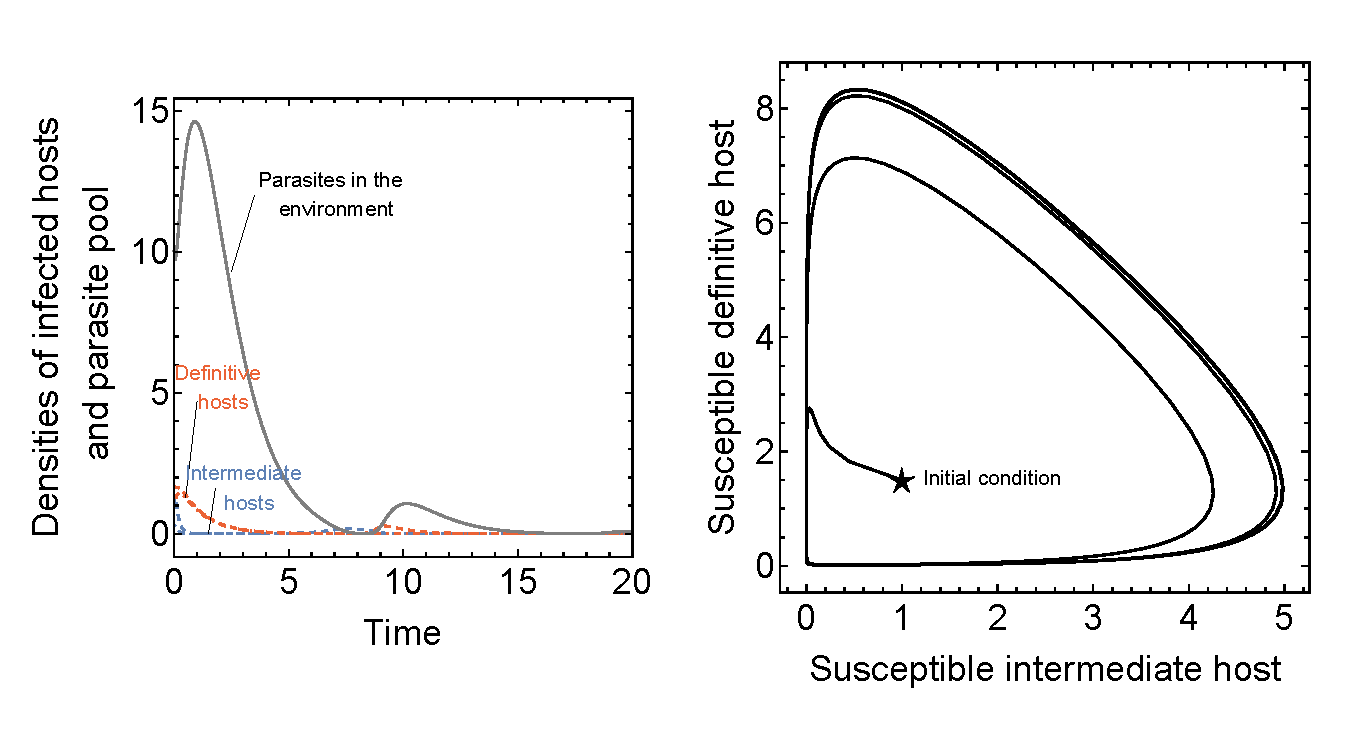
\includegraphics[width=\textwidth]{Figures/diseasefree_linear.pdf}
\caption{Disease-free equilibrium using linear birth function. Solid gray line indicate the density of free-living parasites, blue lines indicate infected intermediate hosts while red lines indicate infected definitive hosts. Dashed lines indicate singly infected hosts while dot-dashed lines indicate doubly infected hosts. Parameter values  $\rho = 1.2, \  d = 0.9, \  r = 2.5, \ \gamma = 2.9, \ \alpha_w =  \alpha_{ww} =  0, \ \beta_w  = 1.5, \ \beta_{ww} = 1.5, \ p = 0.1,  \ c = 1.4, \ \mu = 0.9,  \ \sigma_w = \sigma_{ww} = 0, \ q = 0.01, \  f_w = 6.5, \  f_{ww} = 7.5, \ \delta = 0.9$, $R_0 = 2.233$ } 
\label{fig:diseasefree:linear}
\end{figure}

\subsection*{Non-linear birth function of intermediate hosts}
The non-linear birth function of intermediate hosts is as followed,
\begin{align*}
R(I_w, I_s,I_{ww}) = r I_{total} (1 - k I_{total})
\end{align*}
%
where $k$ is the intraspecific competition coefficient. 
The disease-free equilibrium is as follows
%
\begin{align*}
& I_{s0}^* = \frac{\mu}{c \rho } \\
& D_{s0}^* = \frac{c \rho  (r-d) - k \mu  r}{c \rho ^2}
\end{align*}
%
This equilibrium is stable if,
%
\begin{align*}
& r > d \\
& \frac{2 c \rho  \left(\sqrt{\frac{-d+\mu +r}{\mu }}-1\right)}{r}\leq k < \frac{c \rho  (r-d)}{\mu  r} \\
& \mu >\frac{4 c^2 \rho ^2 r - 4 c^2 d \rho ^2}{4 c k \rho r + k^2 r^2}
\end{align*}

The above conditions suggest that the intrinsic reproduction of intermediate hosts $r$ needs to be greater than their natural mortality rate $d$. 
More importantly, the intraspecific competition coefficient has to be within a range allowing the population to survive.
Finally, the definitive host's natural mortality rate must be sufficiently large. 
Satisfying such conditions, we obtain a stable disease-free equilibrium (Figure \ref{fig:ecotraject:nonlinear}B).

\begin{figure}[!ht]
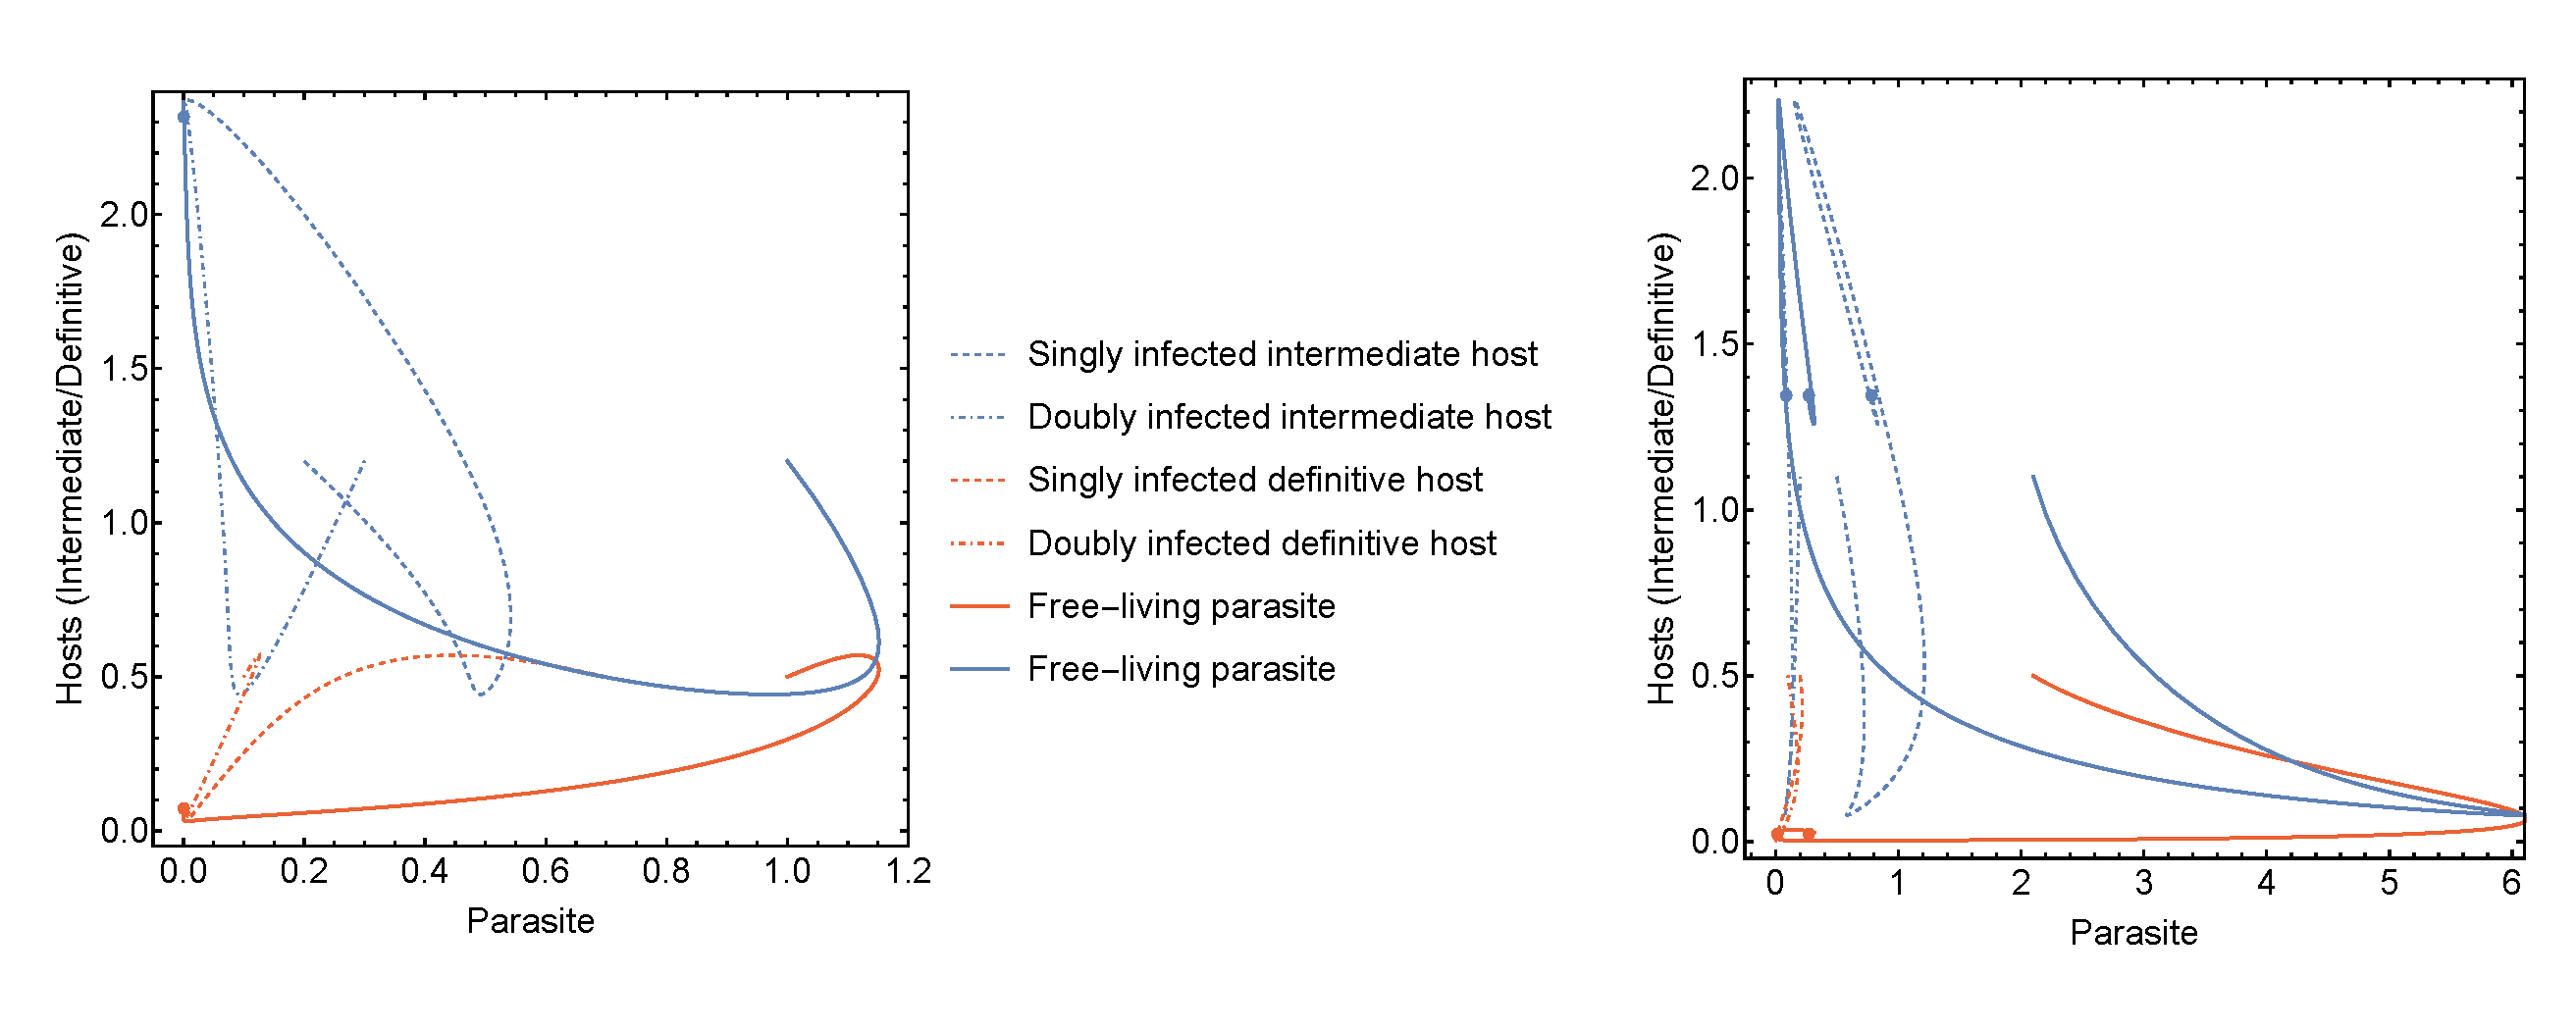
\includegraphics[width=\textwidth]{Figures/ecotraject_nonlinear.pdf}
\caption{Trajectories of parasite and host dynamics. Intermediate hosts represented by blue and definitive host represented by orange. A) Disease free equilibrium where parasite densities at equilibrium is zero. B) Disease stable equilibrium where there are multiple parasite densities which correspond to free parasite pool, singly infected hosts and doubly infected hosts. Fill circles represent stable equilibrium. Parameters for disease free equilibrium $\rho =  1.2, \ d = 0.9, \  r = 2.5, \ \gamma =  2.9, \alpha_w = \alpha_{ww} =  0, \ \beta_w = \beta_{ww} = 1.5, \ p = 0.1, \  c = 1.4, \ \mu = 3.9, \ \sigma_w = \sigma_{ww} = 0, \ q = 0.01, \ f_w = f_{ww} = 7.5, \ \delta = 0.9, \ k = 0.26$. Disease stable equilibrium have the same parameter values except for higher host manipulation $ \beta_w =  \beta_{ww} = 4.5$ and parasite reproduction $ f_w  = f_{ww} = 45$}
\label{fig:ecotraject:nonlinear}
\end{figure}

When a parasite is introduced in the disease-free equilibrium, it spreads if its reproduction ratio $R_0 > 1$. 
Since the expression is complicated, we could not obtain analytical solutions for this inequality without assumptions. 
We assume the same parasite virulence ($\alpha_w = \alpha_{ww}$, $\sigma_w = \sigma_{ww}$), and reproduction in double infection as a linear function concerning reproduction in single infections ($f_{ww} = \epsilon f_w$).
We found that the parasite can establish if its reproduction value in single infection $f_w$ is more significant than a threshold (Figure \ref{fig:bistability}, SI). 
When $\epsilon > 1$, reproduction in double infections is greater than reproduction in single infection, whereas $\epsilon \leq 1$, reproduction in double infections is lower or equal to reproduction in a single infection.
 
Our numerical results show that the parasite reproduction is substantial compared to other parameters (its value is 40 times greater than other parameters), suggesting that trophically transmitted parasites must release many offspring into the environment to persist. 
Interestingly, bistability occurs if the reproduction rate of the parasite in double infections is greater than in the single infection state (Figure \ref{fig:bistability}A, B). 

\begin{figure}[!ht]
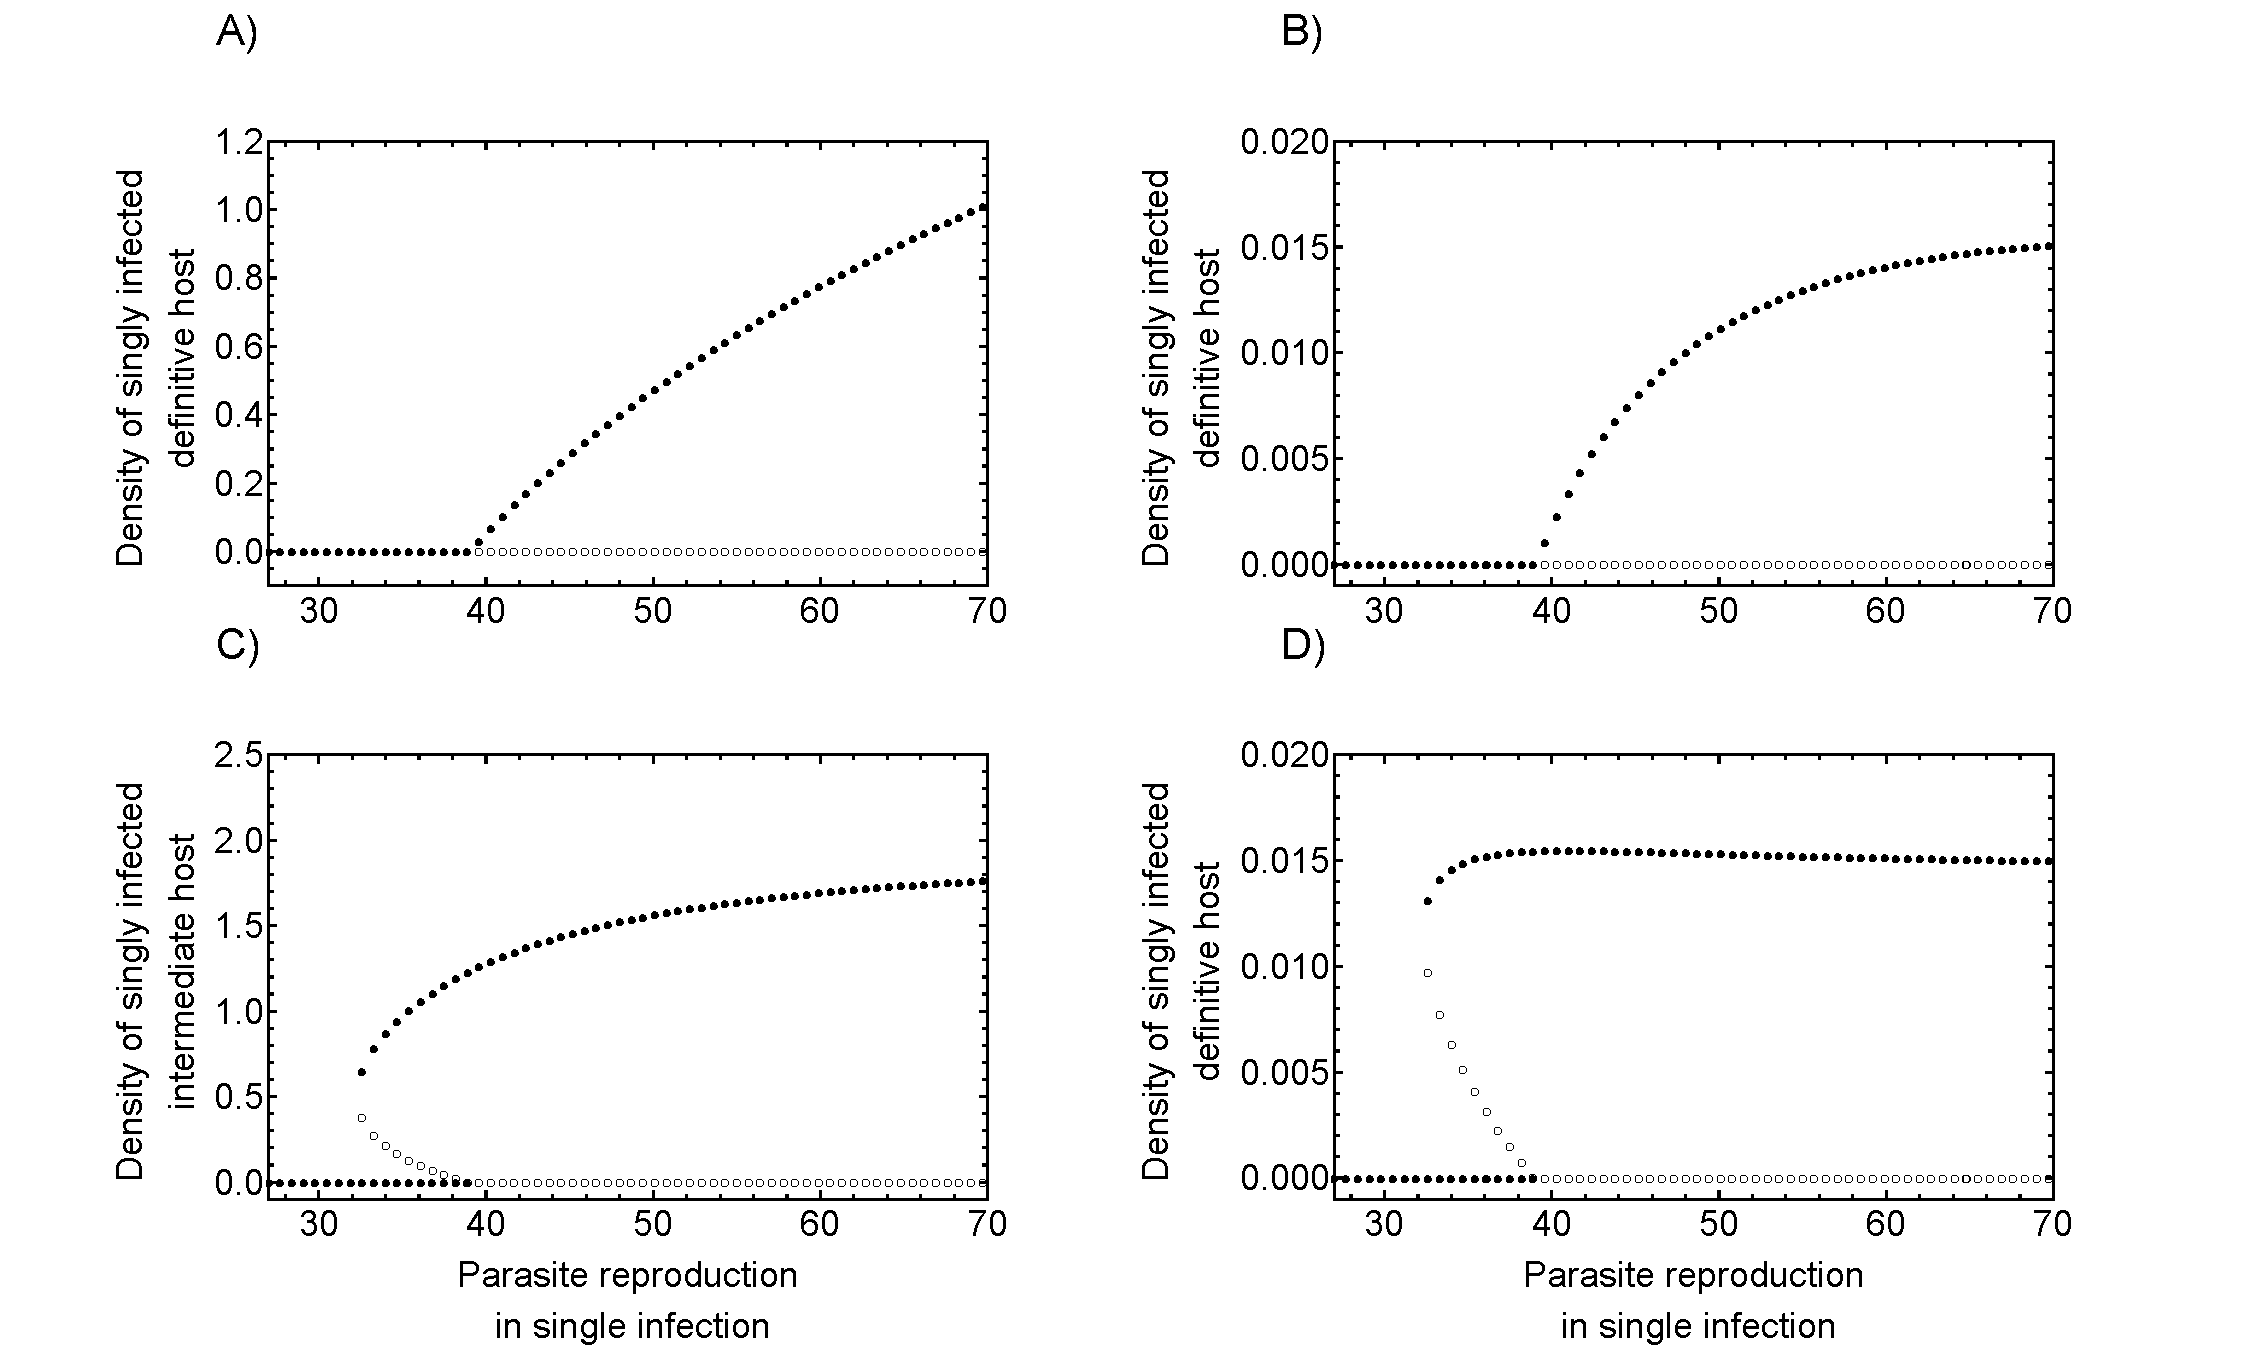
\includegraphics[width = \textwidth]{Figures/bistability.pdf}
\caption{Effect of parasite reproduction on the ecological dynamics. A, B) When reproduction of parasites are the same in singly and doubly infected hosts $\epsilon = 1$. C, D)  When reproduction of parasites in singly infected hosts is four times greater than those in doubly infected hosts $\epsilon = 4$. Filled circles indicate stable equilibrium and open circles indicate unstable equilibrium. Parameter $\rho = 1.2, \  d = 0.9, \  r = 2.5, \ \gamma = 2.9, \ \alpha_w = 0, \ \alpha_ww =  0, \ \beta_w = 1.5, \ \beta_{ww} = 1.5, \ p = 0.1, \  c = 1.4, \ \mu = 3.9,  \ \sigma_w = 0, \ \sigma_{ww} = 0, \  q = 0.01, \ \delta = 0.9, \ k = 0.26$
}
\label{fig:bistability}
\end{figure}

\subsection*{The effect of host manipulation on ecological dynamics}

Host manipulation can be cooperative; two parasites increase the predation rate on intermediate hosts, or $\beta_{ww} > \beta_w$. 
However, it can also be uncooperative; that is, the predation rate on doubly-infected intermediate hosts lower than that on singly-infected ones, or $\beta_{ww} < \beta_w$.
Cooperation in parasite manipulation increases the basic reproduction ratio of the parasite. 
However, if the ability to manipulate the host in a single infection is not strong enough, such cooperation widens the bistable state of the system (Figure \ref{fig:manipR0}). 
Within the bistable region, the basic reproduction ratio is less than one, suggesting that the parasite cannot spread when its manipulative values is within this area of weak manipulation when single and intermediate manipulation when coinfected. 
Parasites that can persist in the population may have weak manipulative activity in a single infection but become much more manipulative in coinfection. 
Likewise, parasites can persist if uncooperative but can manipulate the intermediate hosts effectively when alone.

\begin{figure}
\centering
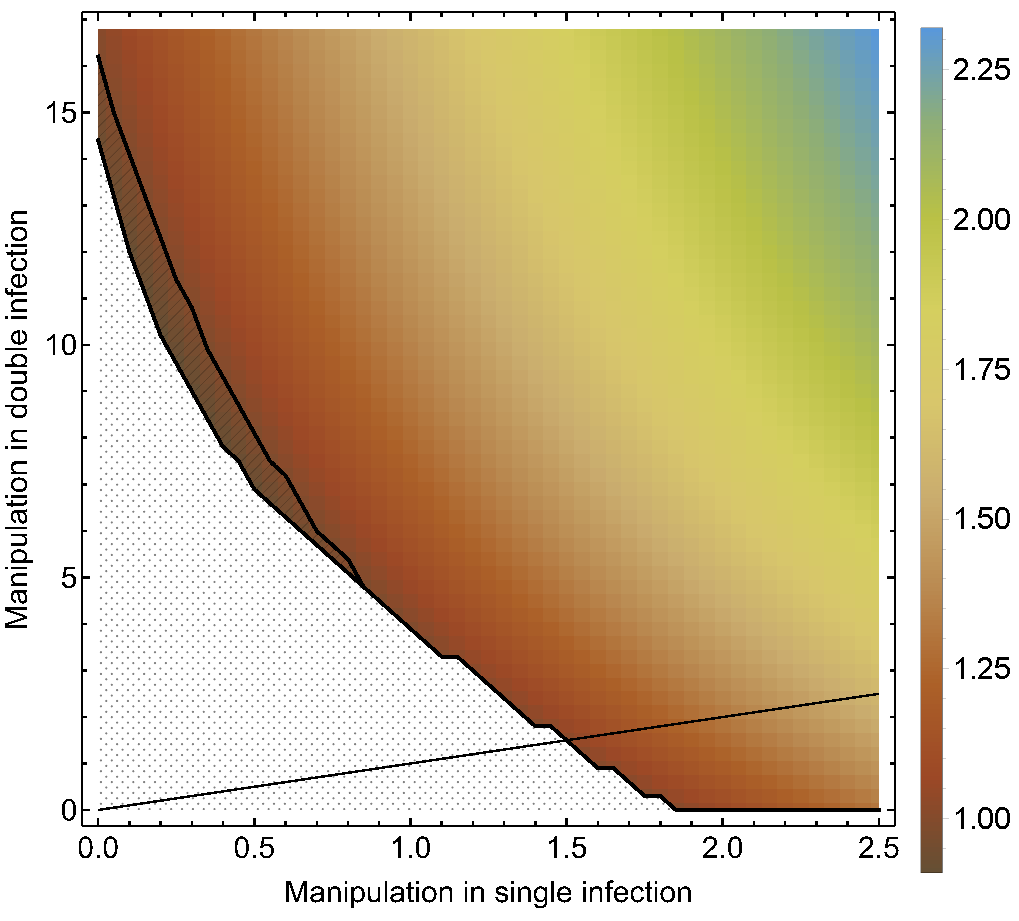
\includegraphics[width=\textwidth]{Figures/manip_bifur_R0.pdf}
\caption{The parasite goes extinct if its manipulative ability is insufficient (dotted area). Bistability region occurs when cooperation in manipulation is intermediate (hatched area). As manipulation in single infection increases, the system only has one stable equilibrium. On the black line, manipulation is indifference between single infection and double infection ($\beta_w = \beta_{ww}$). $R_0 < 1$ in the hatched area indicates that the parasite cannot establish in a disease free prey-predator population.}
\label{fig:manipR0}
\end{figure}

Cooperation between parasites need not be limited to host manipulation. Parasites can cooperate to have a higher reproduction rate in co-infections, i.e. $f_{ww} > f_w$. Likewise, they can also compete with each other for resources, such that reproduction in double infection is smaller than in single infection. Without any assumption on the relationship between manipulative ability and reproduction, we explore all possible combinations of cooperation and sabotage in both manipulation and reproduction. 

Interestingly, higher cooperation in manipulation and reproduction enlarges the area of bistability even though it also shrinks the extinction space (Figure \ref{fig:manipbifur}). 
This suggests that systems in which parasites have much higher manipulative ability and reproduction rate when co-infected than when singly infected are more prone to instability than systems with less cooperative parasites or systems with parasites that sabotage each other in co-infection. 
In other words, having the best of both worlds at the individual level may not benefit the population as a whole.

\begin{figure}[!ht]
\centering
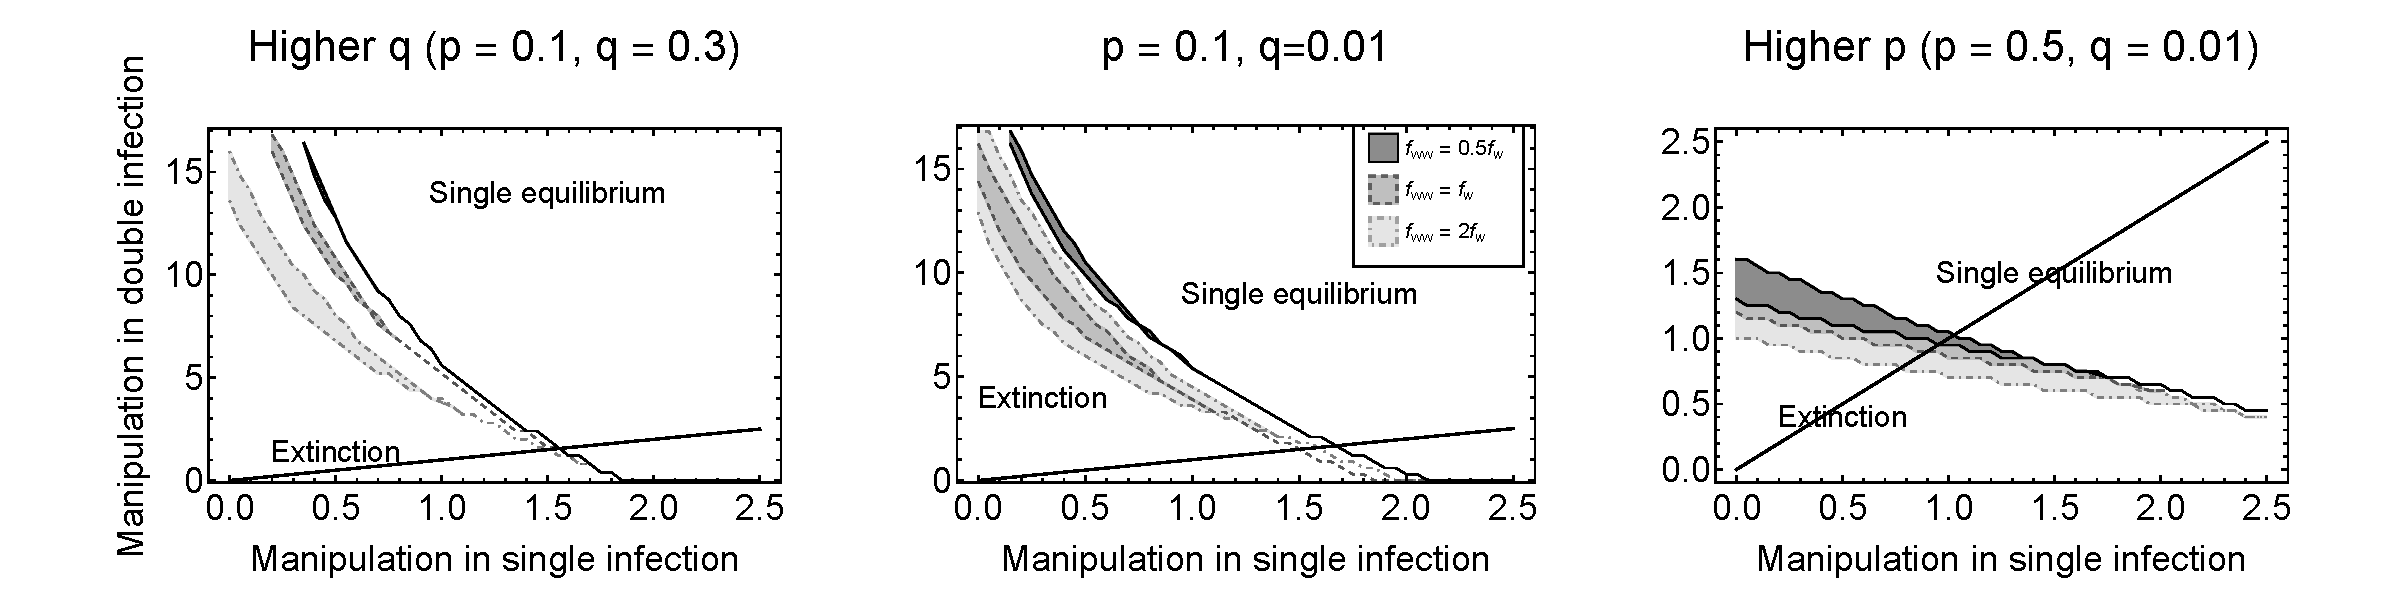
\includegraphics[width=\textwidth]{Figures/manip_bifurcation.pdf}
\caption{Changes of the bistability area (shaded areas) with respect to different reproduction rates in single and double infection (different boundary styles), and varying cotransmission probability. Manipulation is indifference between single infection and double infection on the black line. Common parameter:  $\rho = 1.2, \ d = 0.9, \ r = 2.5, \ \gamma = 2.9, \ \alpha_w = 0, \ \alpha_{ww} = 0, \ p = 0.1, \ c = 1.4, \ \mu = 3.9, \ \sigma_w = 0, \ \sigma_ww = 0, \ q = 0.01, \ \delta = 0.9, \ k = 0.26, \ \epsilon = 0.5$. Parameter for the thick boundary $\epsilon = 0.5, f_w = 36$, the dashed boundary $\epsilon = 1, f_w = 36$, and the dot-dashed boundary $\epsilon = 2, f_w = 35$.}
\label{fig:manipbifur}
\end{figure}

Increasing co-transmission probability $p$ from the parasite pool to intermediate hosts reduces the extinction area, whereas increasing the co-transmission probability $q$ from intermediate hosts to definitive hosts broadens this area. 
When $p$ is high, doubly infected intermediate hosts are more abundant, so cooperation in host manipulation need not be too high to bring the population out of the bi-stability state. 
However, it also means that the singly infected intermediate hosts are few and parasites in single infection need to make more manipulative effort to transmit successfully (Figure \ref{fig:manipbifur}B). 
When $q$ is high, successful transmission to definitive hosts relies on the predation of susceptible definitive hosts on doubly infected intermediate hosts. 
Cooperation in manipulation, therefore, needs to be sufficiently high to avoid bi-stability. 
Sequential transmission is also rarer because the probability of a single infection $1-q$ is low. 
If the number of doubly infected intermediate hosts is low, general transmission from intermediate hosts to definitive hosts is limited, which explains the wide extinction area.

\section*{Discussion \& Conclusion}
Host manipulation is a ubiquitous phenomenon suggested to affect the prey-predator dynamics in trophically transmitted parasites. 
In particular, manipulation in infected intermediate hosts to increase the predation rate of definitive hosts may result in a heavy burden of predator on the intermediate host population, leading to the parasite being more vulnerable to extinction \citep{Hadeler1989, Fenton2006}. 


Our model shows that parasites generally can hardly spread in a cyclic predator-prey system. 
This is an expected result because even though the parasite's basic reproduction ratio $R_0$ is greater than one, it is estimated at the unstable equilibrium (or cyclic equilibrium) of the predator and prey. 
Thus when the density of the prey and predator is at the minimum value of the cycle, the ''effective'' $R_0$ of the parasite can be smaller than one. Another interesting result is that the reproduction value is much larger than other parameter value, which is likely due to the introduction of a free-living parasitic pool. Our model show that in making the system more realistic, we also obtain a more realistic quantitative value for parasitic reproduction.

In our model, non-manipulative parasites cannot persist in the system, and the parasite does not necessarily destabilise the predator-prey system, which may seem to contradict the result of \cite{Rogawa2018}.
In their model, \cite{Rogawa2018} show that a non-manipulative parasite can invade a susceptible prey-predator population and causes the system to cycle. 
The system is stabilised when the parasite becomes manipulative and the stability increases with the manipulative ability.
We suggest that the different results may be due to our introduction of a parasite pool and multiple infections, unlike the model of \cite{Rogawa2018}. There, transmission from definitive host to intermediate host was assumed to be the result of direct contact between the two hosts, and such immediate transmission could directly accelerate the feedback loop between preys and predators. 
Hence, faster predator-prey dynamics occur, which may lead to cyclic dynamics when parasites are introduced.


In our model, host manipulation can destabilise the predator-prey system under particular circumstances and in a different way than the models of \cite{Rogawa2018}. 
In particular, the destabilisation of the system lies in the fact that there is bistability when parasite reproduction in coinfection is boosted. 
In this bistability region, if the system is disturbed (e.g. migration of the intermediate or definitive hosts or predation of intermediate hosts by other predators), then the density of the infected hosts may crash, leading to parasite extinction. 
The bistability region widens as the manipulation in double infection increases, and manipulation in a single infection is insufficient. 
This is because the density of the doubly infected hosts is always much smaller than the singly infected host density. 
It is limited by sequential transmission and a small probability of co-transmission. 
Suppose manipulation in a single infection is not sufficient. 
In that case, the transmission of the parasites depends mainly on the double infection hosts, which is rare. 
So extinction is possible if manipulation in double infection is not sufficiently high.

\cite{Iritani2018} show that manipulative parasites can persist if they can alternate manipulation between enhancing and suppressing predation rate. 
In our model, the parasite cannot switch its manipulative strategy, but we show that sabotage in manipulation when parasites are coinfected almost always leads to the scenario of single stable equilibrium. This result suggests that suppressing manipulation, either by alternating manipulative strategy or by sabotaging the manipulative ability of coinfected parasites, is important in maintaining the parasite population. 

Finally, in this model, we focus on the ecological dynamics of the trophically transmitted parasite. Investigating the evolution of host manipulation is a natural extension. The occurrence of bistability in our model suggests that evolution of host manipulation may drive the parasite population to extinction simply because of the scarcity of the mutant and the Allee effect in the population dynamics. Moreover, if there is no relationship between manipulation and reproduction, the parasite can enhance both values in theory. Yet our model shows that this strategy that seems to reach the best of both worlds make the system even more unstable. Evidently, the course of evolution depends largely on the trade-off between host manipulation and other traits of the parasites such as reproduction, virulence, survivorship in the parasite pool, and so on. This deserves a thorough analyses and should be treated as a separate matter.

%\section*{Conclusion}


%%%%%%%%%%%%%%%%%%%%%
% Acknowledgments
%%%%%%%%%%%%%%%%%%%%%
% You may wish to remove the Acknowledgments section while your paper 
% is under review (unless you wish to waive your anonymity under
% double-blind review) if the Acknowledgments reveal your identity.
% If you remove this section, you will need to add it back in to your
% final files after acceptance.

 \section*{Acknowledgments}
This paper is in memory of Martin Kalbe, an outstanding parasitologist and an exemplary friend and human being.
\cha{Actually I realised we do not cite Martin Kalbe at all.. a bit of a bummer.. I cannot find the bib file that you are using so we can discuss it next time?}
\cha{Phuong?}
Funding from the Max Planck Society if gratefully acknowledged (CSG).

 \section*{Statement of Authorship}
Both authors developed the theory.
P.L.N developed and implemented the computational model.
Both authors wrote the manuscript.
 
\section*{Data and Code Availability}
All data and simulation codes for generating figures are available on 
\cha{hmm we still need to put this on github}
%All data and simulation codes for generating figures are available on \href{https://anonymous.4open.science/r/genedrives_mating-6841/}{Github}   
%(\url{https://anonymous.4open.science/r/genedrives_mating-6841/}).
%% Reseting the counters for equations, figures, tables
%\renewcommand{\theequation}{A\arabic{equation}}
%% redefine the command that creates the equation number.
%\renewcommand{\thetable}{A\arabic{table}}
%\renewcommand{\thefigure}{A\arabic{figure}}
%
%\setcounter{figure}{0}
%\setcounter{equation}{0}  % reset counter 
%\setcounter{table}{0}
%
%\section*{Appendix A}
%
%
%\section*{Appendix B}
%
%
\newpage{}

%%%%%%%%%%%%%%%%%%%%%
% Bibliography
%%%%%%%%%%%%%%%%%%%%%
% You can either type your references following the examples below, or
% compile your BiBTeX database and paste the contents of your .bbl file
% here. The amnatnat.bst style file should work for this---but please
% let us know if you run into any hitches with it!
%
% If you upload a .bib file with your submission, please upload the .bbl
% file as well; this will be required for typesetting.
%
% The list below includes sample journal articles, book chapters, and
% Dryad references.

\bibliographystyle{amnatnat}
%\bibliography{\string~/Bibtex/et.bib}

\begin{thebibliography}{24}
\providecommand{\natexlab}[1]{#1}

\bibitem[{Alizon (2012)}]{Alizon2012}
Samuel Alizon. 2012.
\newblock Parasite co-transmission and the evolutionary epidemiology of
  virulence.
\newblock {\em Evolution}, 67(4):921--933, November 2012.

\bibitem[{Alizon et~al.(2013)Alizon, de~Roode, Michalakis}]{Alizon2013}
Samuel Alizon, Jacobus~C. de~Roode, and Yannis Michalakis. 2013.
\newblock Multiple infections and the evolution of virulence.
\newblock {\em Ecology Letters}, 16(4):556--567, January 2013.

\bibitem[{Alizon and van Baalen(2008)}]{Alizon2008}
Samuel Alizon and Minus van Baalen. 2008.
\newblock Multiple infections, immune dynamics, and the evolution of virulence.
\newblock {\em The American Naturalist}, 172(4):E150--E168, October 2008.

\bibitem[{Benesh(2016)}]{Benesh:2016dj}
Daniel~P Benesh. 2016.
\newblock {Autonomy and integration in complex parasite life cycles.}
\newblock {\em Parasitology}, 143(14):1824 -- 1846, 2016.

\bibitem[{Choisy and de~Roode(2010)}]{Choisy2010}
Marc Choisy and Jacobus~C. de~Roode. 2010.
\newblock Mixed infections and the evolution of virulence: Effects of resource
  competition, parasite plasticity, and impaired host immunity.
\newblock {\em The American Naturalist}, 175(5):E105--E118, May 2010.

\bibitem[{Fenton and Rands(2006)}]{Fenton2006}
A.~Fenton and S.~A. Rands. 2006.
\newblock The impact of parasite manipulation and predator foraging behavior on
  predator - prey communitites.
\newblock {\em Ecology}, 87(11):2832--2841, November 2006.

\bibitem[{Gandon(2018)}]{Gandon2018}
Sylvain Gandon. 2018.
\newblock Evolution and manipulation of vector host choice.
\newblock {\em The American Naturalist}, 192(1):23--34, July 2018.

\bibitem[{Hadeler and Freedman(1989)}]{Hadeler1989}
K.~P. Hadeler and H.~I. Freedman. 1989.
\newblock Predator-prey populations with parasitic infection.
\newblock {\em Journal of Mathematical Biology}, 27(6):609--631, November 1989.

\bibitem[{Hafer and Milinski(2015)}]{Hafer:2015gl}
Nina Hafer and Manfred Milinski. 2015.
\newblock {When parasites disagree: evidence for parasite-induced sabotage of
  host manipulation.}
\newblock {\em Evolution}, 69(3):611 -- 620, 2015.

\bibitem[{Hosack et~al.(2008)Hosack, Rossignol, and van~den Driessche}]{Hosack2008}
Geoffrey~R. Hosack, Philippe~A. Rossignol, and P.~van~den Driessche. 2008.
\newblock The control of vector-borne disease epidemics.
\newblock {\em Journal of Theoretical Biology}, 255(1):16--25, November 2008.

\bibitem[{Hughes(2012)}]{Hughes2012}
David~P Hughes, Jacques Brodeur, and Frederic Thomas. 2012.
\newblock {\em Host Manipulation by Parasites}.
\newblock Oxford University Press, London, England, June 2012.

\bibitem[{Iritani and Sato(2018)}]{Iritani2018}
Ryosuke Iritani and Takuya Sato. 2018.
\newblock Host-manipulation by trophically transmitted parasites: The
  switcher-paradigm.
\newblock {\em Trends in Parasitology}, 34(11):934--944, November 2018.

\bibitem[{Molyneux and Jefferies(1986)}]{molyneux1986}
D.~H. Molyneux and D.~Jefferies. 1986.
\newblock Feeding behaviour of pathogen-infected vectors.
\newblock {\em Parasitology}, 92(3):721–736, 1986.

\bibitem[{Parker et~al.(2003)Parker, Chubb, Roberts, Michaud, and Milinski}]{Parker2003}
G.~A. Parker, J.~C. Chubb, G.~N. Roberts, M.~Michaud, and M.~Milinski. 2003.
\newblock Optimal growth strategies of larval helminths in their intermediate
  hosts.
\newblock {\em Journal of Evolutionary Biology}, 16(1):47--54, January 2003.

\bibitem[{Ripa and Dieckmann(2013)}]{Ripa:Evol:2013}
Jörgen Ripa and Ulf Dieckmann. 2013.
\newblock Mutant invasions and adaptive dynamics in variable environments.
\newblock {\em Evolution}, 67(5):1279--1290, 2013.

\bibitem[{Rogawa et~al.(2018)Rogawa, Ogata, and Mougi}]{Rogawa2018}
Akiyoshi Rogawa, Shigeki Ogata, and Akihiko Mougi. 2018.
\newblock Parasite transmission between trophic levels stabilizes
  predator{\textendash}prey interaction.
\newblock {\em Scientific Reports}, 8(1), August 2018.

\bibitem[{Roger and Bates(2007)}]{Rogers2007}
Matthew~E Rogers and Paul~A Bates. 2007.
\newblock Leishmania manipulation of sand fly feeding behavior results in
  enhanced transmission.
\newblock {\em {PLoS} Pathogens}, 3(6):e91, 2007.

\bibitem[{Roosien et~al.(2013)Roosien, Gomulkiewicz, Ingwell, Bosque-Perez, Rajabaskar, and Eigenbrode}]{Roosien2013}
Bryan~K. Roosien, Richard Gomulkiewicz, Laura~L. Ingwell, Nilsa~A. 2013.
  Bosque-P{\'{e}}rez, Dheivasigamani Rajabaskar, and Sanford~D. Eigenbrode.
\newblock Conditional vector preference aids the spread of plant pathogens:
  Results from a model.
\newblock {\em Environmental Entomology}, 42(6):1299--1308, December 2013.

\bibitem[{Seppala and Jokela(2008)}]{Seppl2008}
Otto Seppala and Jukka Jokela. 2008.
\newblock Host manipulation as a parasite transmission strategy when
  manipulation is exploited by non-host predators.
\newblock {\em Biology Letters}, 4(6):663--666, August 2008.

\bibitem[{van Baalen and Sabelis(1995)}]{vanBaalen1995}
Minus van Baalen and Maurice~W. Sabelis. 1995.
\newblock The dynamics of multiple infection and the evolution of virulence.
\newblock {\em The American Naturalist}, 146(6):881--910, December 1995.

\bibitem[Vickery and Poulin(2009)]{Vickery2009}
William~L. Vickery and Robert Poulin. 2009.
\newblock The evolution of host manipulation by parasites: a game theory
  analysis.
\newblock {\em Evolutionary Ecology}, 24(4):773--788, November 2009.

\bibitem[Wedekind and Milinski(1996)]{Wedekind1996}
C.~Wedekind and M.~Milinski. 1996.
\newblock Do three-spined sticklebacks avoid consuming copepods, the first
  intermediate host of \textit{Schistocephalus solidus}? - an experimental
  analysis of behavioural resistance.
\newblock {\em Parasitology}, 112(4):371--383, April 1996.

\bibitem[{Zimmer(2001)}]{zimmer:book:2001}
Carl Zimmer. 2001.
\newblock {\em {Parasite Rex: Inside the Bizarre World of Nature's Most
  Dangerous Creatures}}.
\newblock Atria Books, 2001.

\bibitem[{Hurford et~al(2009)Hurford, Cownden and Day}]{Hurford2009}
Amy Hurford, Daniel Cownden and Troy Day
\newblock Next-generation tools for evolutionary invasion analyses
\newblock {\em Journal of The Royal Society Interface}, 45(7):561--571, December 2009.

\bibitem[{Diekmann et~al(2009)Diekmann, Heesterbeek and Roberts}]{Diekmann2009}O. Diekmann, J. A. P. Heesterbeek and M. G. Roberts
\newblock The construction of next-generation matrices for compartmental epidemic models
\newblock {\em Journal of The Royal Society Interface}, 47(7):873--885, November 2009.

\bibitem[{Diekmann et~al(1990)Diekmann, Heesterbeek and Metz}]{Diekmann1990}O. Diekmann, J.A.P. Heesterbeek and J.A.J. Metz
\newblock On the definition and the computation of the basic reproduction ratio R0 in models for infectious diseases in heterogeneous populations
\newblock {\em Journal of Mathematical Biology}, 28(4), June 1990.

\bibitem[Lotka (1920)]{Lotka1920}Alfred J. Lotka
\newblock Analytical Note on Certain Rhythmic Relations in Organic Systems
\newblock {\em Proceedings of the National Academy of Sciences}, (7)6:410--415, July 1920
\end{thebibliography}

\newpage{}

\section*{Tables}
\renewcommand{\thetable}{\arabic{table}}
\setcounter{table}{0}

\begin{table}[h]
%\caption{Examples of natural drive elements with properties simulated in this study.}
%\label{Table:Driveelements}
%\centering
%\begin{tabular}{lllll}\hline
%Species & Drive element & Drive type \& parameters & Ecological properties
% \\ \hline
%\textit{Tribolium castaneum}  & Medea & Viability drive $d$ & Probably low k, highly \\
%  & & & polyandrous\\
 %   & & & \cite{pai:EntoEA:2020} \\
%\textit{Drosophila melanogaster}  & Selfish Segregation  & Distortion drive
%$p$,$c$ & Probably low k, Polyandry \\ 
%& Distorter (SD) & & with some re-mating \\
%& & & latency \cite{singh:CurrSci:2004}\\
%\textit{Mus musculus}  & t-haplotype & Distortion drive
%$p$,$c$ & Probably low k, \\ 
%& & & Polyandry ($r=2,$, \\ 
%& & & \cite{birand:MolEcol:2022}) \\ \hline 
%\end{tabular}
%\bigskip{}
%\\
%{\footnotesize Note: Table titles should be short. Further details should go in a `notes' area after the tabular environment, like this. $^a$ Published the first description of \textit{Dimetrodon}.}
\end{table}
%
\newpage{}

\section*{Figure legends}

\renewcommand{\thefigure}{\arabic{figure}}
\setcounter{figure}{0}
%%

%\begin{figure}[h!]
 %   \centering
% \includegraphics[width=0.65\columnwidth]{figure1.eps}
 %   \caption{\textbf{Pictorial representation of the three mating complexities: mate-choice, mating network, and mating system that can affect gene drive's population dynamics.}}
%    \label{fig:fig1}    
%\end{figure}
%%


% \subsection*{figure legends for Appendices}

\renewcommand{\thefigure}{A\arabic{figure}}
\setcounter{figure}{0}


\end{document}
